\scanpage{56}
% archive sheet number: 55
\margin{[\unsure{Sous rés.|Sans rés.} des questions de dégénérescences)}
$K^*$ \deleted{\unsure{complexe}} objet cosimplicial dans une catégorie abélienne $\unsure{\mathcal C|C}$

C'est donc un \deleted{objet} $\mathcal C$-module gradué sur l'anneau gradué $S$ engendré par les $\partial_i^n$, \deleted{$\unsure{s_i^n|\sigma_i^n}$} \inserted{$(0\leq i\leq n+1)$} avec les relations qu'on sait. \deleted{\unsure{On va}} On va y introduire les \uline{relations}
\[
\partial_i^n=0\qquad\text{pour}\quad1\leq i\leq n
\]
\margin{$\partial_i^n:\Delta^n\longrightarrow\Delta^{n+1}$\par $0\leq i\leq n+1$}

\unsure{donc considérons|en considérant} dans chaque $K^n$ le sous-objet somme des $K^i\longrightarrow K^n$, où \deleted{$K^i$} $i<n$ et où
\[
\deleted{\left\{\begin{aligned}
&\partial_i^n K^{n-1}&&1\leq i\leq n\\
&\unsure{u_2|u}\partial_i^{n-1}K^{n-2}&&1\leq i\leq n\\
&\text{--}\\
&u\quad K^0
\end{aligned}\right.}
\]
$K^i\longrightarrow K^n$ est une opération simpliciale qui correspond à une application \unsure{strictement} croissante de $\underline\Delta^i$ dans $\underline\Delta^n$ qui \uline{n'est pas d'un \unsure{seul} tenant}. On \unsure{trouve|forme} un $K'^n\subset K^n$, et évidemment on a ainsi un \uline{co-\deleted{\unsure{complexe}}objet simplicial} \inserted{$K'^*$} de $K^*$

\diagram{\begin{tikzcd}[ampersand replacement=\&]
\deleted{\overset{\bullet}{x_0}\leq x_1\quad\unsure{x_{n-1}}\leq\overset{\bullet}{x_n}}\arrow[r,no head]\&\\
(x_0,x_1,x_{\unsure{n|2}})\arrow[d]\&\\
(x_0,x_{\unsure{2|n}})\&
\end{tikzcd}}
\diagram{\begin{tikzcd}[ampersand replacement=\&]
A_{(x_0x_1x_2)}\\
A_{[x_0,x_2]}\arrow[u]
\end{tikzcd}}
\figure{\begin{tikzpicture}\draw (0,.15) to[out=-15,in=200] (2.6,.8) to[out=20,in=180] (3.1,.85);\end{tikzpicture}}
\diagram{\begin{tikzcd}[ampersand replacement=\&,column sep=large]
\&\displaystyle\sum A_{[x_0,x_1,x_2]}\&\&\\
\displaystyle\sum A_{[x_0,x_1]}\&\displaystyle\sum A_{[x_1,x_2]}\& A_{[x_0,x_2]}\arrow[ul]\&\\
\underline{A_{[x_0]}}\arrow[u]\arrow[rrr,bend right=45]\&\underline{A_{[x_1]}}\arrow[ul]\arrow[u]\&\underline{A_{[x_2]}}\arrow[u]\&{}
\end{tikzcd}}
\figure{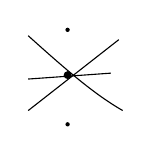
\begin{tikzpicture}[scale=.5]
\draw (-1,1)..controls (0,.1) and (.7,-.5)..(1.4,-.9);\draw (-1,-.9)--(1.3,.9);\draw (-1,-.1)--(1.1,.05);
\fill (0,0) circle (.1);\fill (0,1.15) circle (.055);\fill (0,-1.25) circle (.055);
\end{tikzpicture}}

\[A_{[x_0\quad x_1}\]
\[x_0,x_2\]
\[A_{[x_0,x_2]}\qquad\partial_1^1 A_{[x_0,x_2]}\]
\diagram{\begin{tikzcd}[ampersand replacement=\&]
\unsure{0|o}\&K''\arrow[l]\arrow[r,no head]\&K'\arrow[r,no head]\&K\arrow[r]\&0
\end{tikzcd}}

\figure{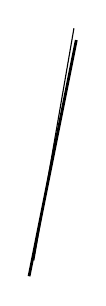
\begin{tikzpicture}\draw[line width=1pt] (0,0)--(.6,3);\draw (.06,.2)--(.57,3.15);\end{tikzpicture}}
